\documentclass[10pt]{amsart}
\usepackage{amsmath}
\usepackage{amssymb,amscd}
\usepackage{tikz,tkz-euclide}
\usepackage{tikz-cd}
\usetikzlibrary{arrows}
\usepackage{tikz-3dplot}
\usepackage{color}
\usepackage[colorlinks=true,linkcolor=darkblue, urlcolor=darkblue, citecolor=darkblue]{hyperref}

\begin{document}

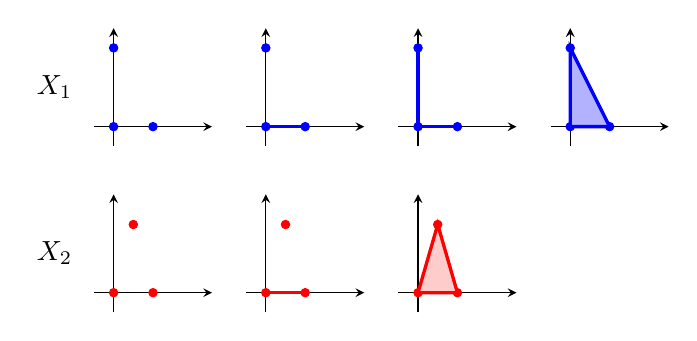
\begin{tikzpicture}
\begin{scope}[scale=0.5]
\node at (-1.5, 1) {$X_1$};
\draw[-stealth] (-0.5,0)--(2.5,0);
\draw[-stealth] (0,-0.5)--(0,2.5);
\draw[fill=blue, blue] (0,0) circle (3pt);
\draw[fill=blue, blue] (1,0) circle (3pt);
\draw[fill=blue, blue] (0,2) circle (3pt);

\begin{scope}[xshift=110]
\draw[-stealth] (-0.5,0)--(2.5,0);
\draw[-stealth] (0,-0.5)--(0,2.5);
\draw[fill=blue, blue] (0,0) circle (3pt);
\draw[fill=blue, blue] (1,0) circle (3pt);
\draw[fill=blue, blue] (0,2) circle (3pt);
\draw[very thick, blue] (0,0)--(1,0);
\end{scope}

\begin{scope}[xshift=220]
\draw[-stealth] (-0.5,0)--(2.5,0);
\draw[-stealth] (0,-0.5)--(0,2.5);
\draw[fill=blue, blue] (0,0) circle (3pt);
\draw[fill=blue, blue] (1,0) circle (3pt);
\draw[fill=blue, blue] (0,2) circle (3pt);
\draw[very thick, blue] (0,0)--(1,0);
\draw[very thick, blue] (0,0)--(0,2);
\end{scope}

\begin{scope}[xshift=330]
\draw[-stealth] (-0.5,0)--(2.5,0);
\draw[-stealth] (0,-0.5)--(0,2.5);
\draw[fill=blue, blue] (0,0) circle (3pt);
\draw[fill=blue, blue] (1,0) circle (3pt);
\draw[fill=blue, blue] (0,2) circle (3pt);
\draw[very thick, blue, fill=blue!30] (0,0)--(1,0)--(0,2)--cycle;
\end{scope}

\begin{scope}[yshift=-120]
\node at (-1.5, 1) {$X_2$};
\draw[-stealth] (-0.5,0)--(2.5,0);
\draw[-stealth] (0,-0.5)--(0,2.5);
\draw[fill=red, red] (0,0) circle (3pt);
\draw[fill=red, red] (1,0) circle (3pt);
\draw[fill=red, red] (1/2,1.7320508076) circle (3pt);

\begin{scope}[xshift=110]
\draw[-stealth] (-0.5,0)--(2.5,0);
\draw[-stealth] (0,-0.5)--(0,2.5);
\draw[fill=red, red] (0,0) circle (3pt);
\draw[fill=red, red] (1,0) circle (3pt);
\draw[fill=red, red] (1/2,1.7320508076) circle (3pt);
\draw[very thick, red] (0,0)--(1,0);
\end{scope}

\begin{scope}[xshift=220]
\draw[-stealth] (-0.5,0)--(2.5,0);
\draw[-stealth] (0,-0.5)--(0,2.5);
\draw[fill=red, red] (0,0) circle (3pt);
\draw[fill=red, red] (1,0) circle (3pt);
\draw[fill=red, red] (1/2,1.7320508076) circle (3pt);
\draw[very thick, red, fill=red!20] (0,0)--(1/2,1.7320508076)--(1,0)--cycle;
\end{scope}
\end{scope}
\end{scope}
\end{tikzpicture}

\end{document}